% B.Tech mini-project report: QAOA-Based Economic Load Dispatch
% Compile on Overleaf with pdfLaTeX (upload the whole report/ folder).
\documentclass[12pt,a4paper,oneside]{report}

\usepackage[a4paper,left=1.5in,right=1in,top=1in,bottom=1in]{geometry}
\usepackage[T1]{fontenc}
\usepackage{lmodern}
\usepackage{amsmath,amssymb}
\usepackage{graphicx}
\usepackage{booktabs}
\usepackage{array}
\usepackage{float}
\usepackage{caption}
\usepackage{setspace}
\usepackage{fancyhdr}
\usepackage{titlesec}
\usepackage{enumitem}
\usepackage{xcolor}
\usepackage{listings}
\usepackage[hidelinks]{hyperref}

\graphicspath{{figures/}}
\onehalfspacing
\captionsetup{font=small,labelfont=bf}
\setlist{itemsep=2pt,topsep=4pt}
\setlength{\tabcolsep}{4pt}

\titleformat{\chapter}[display]{\normalfont\Large\bfseries\centering}{CHAPTER \thechapter}{8pt}{\LARGE}
\titlespacing*{\chapter}{0pt}{-20pt}{24pt}

\pagestyle{fancy}
\fancyhf{}
\fancyhead[L]{\small QAOA-Based Economic Load Dispatch}
\fancyhead[R]{\small Dept. of EEE, RGUKT Nuzvid}
\fancyfoot[C]{\thepage}
\renewcommand{\headrulewidth}{0.4pt}
\fancypagestyle{plain}{\fancyhf{}\fancyfoot[C]{\thepage}\renewcommand{\headrulewidth}{0pt}}

\lstset{basicstyle=\ttfamily\small,columns=fullflexible,frame=single,breaklines=true}

\newcommand{\PD}{P_{\mathrm{D}}}
\newcommand{\PL}{P_{\mathrm{L}}}

\begin{document}

\pagenumbering{roman}
% ---------------- Title page ----------------
\begin{titlepage}
\centering
{\Large\bfseries QAOA-BASED ECONOMIC LOAD DISPATCH\\[4pt] USING QUBO FORMULATION\par}
\vspace{0.8cm}
{\large A Mini Project Report submitted in partial fulfilment of the\\ requirements for the award of the degree of\par}
\vspace{0.4cm}
{\large\bfseries BACHELOR OF TECHNOLOGY\\ in\\ ELECTRICAL AND ELECTRONICS ENGINEERING\par}
\vspace{0.8cm}
{\large Submitted by\par}
\vspace{0.3cm}
\begin{tabular}{ll}
J. Karthikeya & (Roll No: \rule{3cm}{0.4pt})\\
A. Krishna Chaitanya & (Roll No: \rule{3cm}{0.4pt})\\
N. Ramesh & (Roll No: \rule{3cm}{0.4pt})\\
M. Harika & (Roll No: \rule{3cm}{0.4pt})\\
\end{tabular}
\vspace{0.8cm}

{\large Under the guidance of\\[4pt] \bfseries B. Madhusudhan Rao\par}
\vfill
% Place the college logo here if required: \includegraphics[width=3cm]{rgukt_logo}
{\large\bfseries DEPARTMENT OF ELECTRICAL AND ELECTRONICS ENGINEERING\\
RAJIV GANDHI UNIVERSITY OF KNOWLEDGE TECHNOLOGIES\\
NUZVID, ANDHRA PRADESH\par}
\vspace{0.3cm}
{\large NOVEMBER 2026\par}
\end{titlepage}

% ---------------- Certificate ----------------
\chapter*{Certificate}
\addcontentsline{toc}{chapter}{Certificate}
This is to certify that the mini project report entitled \textbf{``QAOA-Based Economic Load Dispatch Using QUBO Formulation''} is a bonafide record of the work carried out by \textbf{J.~Karthikeya, A.~Krishna Chaitanya, N.~Ramesh and M.~Harika} in partial fulfilment of the requirements for the award of the degree of Bachelor of Technology in Electrical and Electronics Engineering at Rajiv Gandhi University of Knowledge Technologies, Nuzvid, during the academic year 2026--27, under my supervision and guidance.

\vspace{3cm}
\noindent
\begin{minipage}[t]{0.48\textwidth}
\rule{5cm}{0.4pt}\\
\textbf{B. Madhusudhan Rao}\\
Project Guide\\
Department of EEE\\
RGUKT Nuzvid
\end{minipage}\hfill
\begin{minipage}[t]{0.48\textwidth}\raggedleft
\rule{5cm}{0.4pt}\\
\textbf{Head of the Department}\\
Department of EEE\\
RGUKT Nuzvid
\end{minipage}

% ---------------- Declaration ----------------
\chapter*{Declaration}
\addcontentsline{toc}{chapter}{Declaration}
We hereby declare that the work presented in this mini project report entitled \textbf{``QAOA-Based Economic Load Dispatch Using QUBO Formulation''} has been carried out by us under the guidance of B.~Madhusudhan Rao, Department of Electrical and Electronics Engineering, RGUKT Nuzvid. All data, methods and results taken from other sources have been acknowledged and cited. The work has not been submitted elsewhere for the award of any other degree.

\vspace{2.5cm}
\noindent
\begin{tabular}{@{}p{0.5\textwidth}p{0.4\textwidth}@{}}
J. Karthikeya & \rule{4cm}{0.4pt}\\[14pt]
A. Krishna Chaitanya & \rule{4cm}{0.4pt}\\[14pt]
N. Ramesh & \rule{4cm}{0.4pt}\\[14pt]
M. Harika & \rule{4cm}{0.4pt}\\
\end{tabular}

\vspace{1cm}
\noindent Place: Nuzvid\\
Date: \rule{3cm}{0.4pt}

% ---------------- Acknowledgement ----------------
\chapter*{Acknowledgement}
\addcontentsline{toc}{chapter}{Acknowledgement}
We express our sincere gratitude to our project guide, \textbf{B.~Madhusudhan Rao}, Department of Electrical and Electronics Engineering, for the guidance, encouragement and constructive feedback given throughout this project.

We thank the Head of the Department and all faculty members of the Department of EEE, RGUKT Nuzvid, for the facilities and support provided. We also thank the review panel for their suggestions during the project reviews.

We acknowledge IBM Quantum for free access to quantum hardware through the IBM Quantum Platform Open plan, and the developers of Qiskit, SciPy, MATPOWER and PYPOWER, whose open-source tools made this work possible.

\vspace{1.5cm}
\noindent\hfill J.~Karthikeya\\
\hspace*{\fill} A.~Krishna Chaitanya\\
\hspace*{\fill} N.~Ramesh\\
\hspace*{\fill} M.~Harika

% ---------------- Abstract ----------------
\chapter*{Abstract}
\addcontentsline{toc}{chapter}{Abstract}
Economic load dispatch (ELD) allocates the system load among committed generators so that total fuel cost is minimised while power balance and generator limits are met. This project studies whether the Quantum Approximate Optimization Algorithm (QAOA), a variational algorithm for near-term quantum computers, can solve ELD once it is written as a quadratic unconstrained binary optimisation (QUBO) problem.

The 6-bus, 3-generator Wood--Wollenberg system with the 12-period load profile of Prada (2017) is used as the test case. Each generator output is encoded with four binary variables, giving a 12-qubit QUBO in which the power-balance constraint enters as a quadratic penalty. The penalty weight $A = 20$ was selected by a sweep over four values. The QUBO is mapped to an Ising Hamiltonian and solved with QAOA at depths $p = 1$ to $4$, trained with the conditional value-at-risk (CVaR) objective and INTERP initialisation. The five lowest-energy sampled bitstrings are refined by a bounded classical step to remove the residual power mismatch.

The hybrid QAOA dispatch is within 0.041\,\% of the SLSQP optimum in every period (total cost \$43{,}173.88/h against \$43{,}171.05/h), and QAOA sampled the exact QUBO optimum in all 12 periods. At $p = 4$ the optimal dispatch is measured 10.2 times more often than under uniform sampling. Over 240 runs per method, QAOA with refinement succeeded in 100\,\% of cases against 92.5\,\% for simulated annealing on the same QUBO with the same evaluation budget and refinement; particle swarm optimisation and a genetic algorithm reach the continuous optimum when the dependent-unit method is used, but only 13.8\,\% and 7.5\,\% of runs succeed with a plain penalty. On the 156-qubit IBM \texttt{ibm\_marrakesh} processor, a 6-qubit instance found the optimum 2.4 times more often than random sampling, while gate noise removed most of the gain at 9 qubits.

The study is extended to transmission losses using B-coefficients derived from the network, and every dispatch is checked with a Newton--Raphson AC load flow validated against PYPOWER. The work shows that QAOA solves ELD accurately but does not give a speed-up over classical methods for a problem of this size; its natural application is larger binary problems such as unit commitment.

\vspace{0.5cm}
\noindent\textbf{Keywords:} Economic load dispatch, QAOA, QUBO, Ising model, quantum computing, CVaR, Newton--Raphson load flow.


\tableofcontents
\listoffigures
\listoftables
\chapter*{List of Abbreviations and Symbols}
\addcontentsline{toc}{chapter}{List of Abbreviations and Symbols}
\begin{tabular}{@{}p{0.22\textwidth}p{0.72\textwidth}@{}}
\toprule
ELD & Economic Load Dispatch\\
QAOA & Quantum Approximate Optimization Algorithm\\
QUBO & Quadratic Unconstrained Binary Optimisation\\
CVaR & Conditional Value-at-Risk\\
SLSQP & Sequential Least-Squares Quadratic Programming\\
PSO & Particle Swarm Optimisation\\
GA & Genetic Algorithm\\
SA & Simulated Annealing\\
SBX & Simulated Binary Crossover\\
NR & Newton--Raphson (load flow)\\
PTDF & Power Transfer Distribution Factor\\
NISQ & Noisy Intermediate-Scale Quantum\\
COBYLA & Constrained Optimisation BY Linear Approximation\\
\midrule
$P_i$ & Real power output of generator $i$ (MW)\\
$a_i, b_i, c_i$ & Cost coefficients of generator $i$ (\$/MW$^2$h, \$/MWh, \$/h)\\
$\PD$, $\PL$ & Total demand and transmission loss (MW)\\
$\lambda$ & Incremental cost (\$/MWh)\\
$x_{ik}$ & Binary variable $k$ of generator $i$\\
$\Delta P_i$ & Encoding step of generator $i$ (MW)\\
$A$ & Penalty weight for power balance (\$/MW$^2$h)\\
$H_C$, $H_M$ & Cost and mixer Hamiltonians\\
$Z_j$, $X_j$ & Pauli $Z$ and $X$ operators on qubit $j$\\
$p$ & QAOA depth (number of layers)\\
$\gamma_\ell, \beta_\ell$ & QAOA angles of layer $\ell$\\
$\alpha$ & CVaR tail fraction\\
$B$, $B_0$, $B_{00}$ & Loss-formula coefficients\\
\bottomrule
\end{tabular}


\cleardoublepage
\pagenumbering{arabic}
\chapter{Introduction}

\section{Background}
A power system must supply a load that changes from hour to hour. For every load level, the operator decides how much power each committed generating unit should produce. Because the units have different fuel costs, the way the load is shared changes the total operating cost. \emph{Economic load dispatch} (ELD) is the problem of choosing these outputs so that the total fuel cost is as small as possible, while generation equals demand plus losses and every unit stays inside its limits \cite{wood2014}. ELD is solved every few minutes in a real control centre and is a core topic of power-system operation.

For units with quadratic cost curves and no other constraints, ELD is a convex problem: the classical equal-incremental-cost ($\lambda$-iteration) method and general solvers such as sequential quadratic programming find the global optimum in milliseconds. Practical extensions such as unit commitment (on/off decisions), prohibited operating zones and valve-point effects make the problem non-convex or combinatorial, and those versions are where new optimisation methods are tested.

\section{Quantum computing and QAOA}
Quantum computers store information in qubits, which can be in superpositions of 0 and 1. A register of $n$ qubits can therefore represent a superposition of all $2^n$ bitstrings at once. Present devices are \emph{noisy intermediate-scale quantum} (NISQ) processors with tens to hundreds of qubits and limited circuit depth.

The Quantum Approximate Optimization Algorithm (QAOA), proposed by Farhi, Goldstone and Gutmann in 2014 \cite{farhi2014}, is designed for such devices. It prepares a parameterised quantum state whose measurement favours low-cost bitstrings of a combinatorial problem, and a classical optimiser tunes the parameters. QAOA solves problems written as a \emph{quadratic unconstrained binary optimisation} (QUBO), which is equivalent to finding the ground state of an Ising Hamiltonian \cite{lucas2014}.

\section{Motivation}
Several studies have proposed quantum and quantum-inspired methods for power-system optimisation, including economic dispatch \cite{han2024,jing2023,wang2024}. Before such methods can be trusted for larger, harder problems, they must be shown to work correctly on a problem whose true answer is known. ELD on a small system is such a problem: the classical optimum is available exactly, so the accuracy of the quantum method can be measured rather than assumed. This project carries out that test carefully and reports both what QAOA achieves and where it falls short.

\section{Objectives}
\begin{enumerate}
\item Formulate ELD of the 6-bus, 3-generator system as a QUBO using binary encoding of generator outputs and a quadratic power-balance penalty, and map it to an Ising Hamiltonian.
\item Solve the 12-qubit problem with QAOA for all 12 load periods, and study the effect of circuit depth.
\item Refine the QAOA samples with a bounded classical step to obtain dispatches that meet demand exactly (hybrid QAOA).
\item Benchmark the result against SLSQP, $\lambda$-iteration and standard heuristics (PSO, GA, simulated annealing) using a common success criterion.
\item Execute the QAOA circuit on real IBM quantum hardware.
\item Extend the study to transmission losses and check all dispatches with an AC Newton--Raphson load flow.
\end{enumerate}

\section{Scope and limitations}
The study is limited to static, single-period ELD with quadratic costs for each of the 12 periods; ramp-rate coupling between periods, unit commitment and reserves are outside its scope. The full 12-qubit QAOA is evaluated on a classical simulator; real hardware is used for 6- and 9-qubit versions. Line flow limits are not enforced in the dispatch, but they are checked afterwards with the load flow.

\section{Organisation of the report}
Chapter~2 reviews related work. Chapter~3 describes the ELD problem and the test system. Chapter~4 develops the QUBO formulation and the QAOA method. Chapter~5 describes the software implementation. Chapter~6 presents results on the simulator, the comparison with standard algorithms and the hardware experiment. Chapter~7 covers transmission losses and AC validation. Chapter~8 concludes the report and outlines future work.

\chapter{Literature Review}

\section{Classical economic dispatch}
The classical treatment of ELD is given by Wood, Wollenberg and Sheblé \cite{wood2014}. With quadratic costs $C_i(P_i) = a_iP_i^2 + b_iP_i + c_i$, the optimality condition is that every unit not at a limit operates at the same incremental cost $\lambda = dC_i/dP_i$; the $\lambda$-iteration method searches for this common value. Transmission losses are commonly represented by Kron's loss formula $\PL = P^\top B P + B_0^\top P + B_{00}$, whose coefficients are derived from the network. General nonlinear programming solvers, such as SLSQP \cite{kraft1988}, solve the same problem directly and handle additional constraints.

\section{Heuristic methods for ELD}
Population-based heuristics are widely used for non-convex dispatch. Gaing \cite{gaing2003} applied particle swarm optimisation (PSO) to ELD with generator constraints and handled the power-balance equality by computing one ``dependent'' unit from the others, which keeps every candidate exactly balanced. The inertia-weight PSO of Shi and Eberhart \cite{shi1998} is the usual variant. Real-coded genetic algorithms with simulated binary crossover (SBX) \cite{deb1995} and simulated annealing \cite{kirkpatrick1983} are other standard choices. These methods are used in this project as benchmarks.

\section{QUBO and Ising formulations}
Lucas \cite{lucas2014} showed how many NP problems can be written as Ising models: binary decision variables become spins, objectives become linear and quadratic terms, and constraints become quadratic penalties. The substitution $x = (1 - z)/2$ converts a QUBO in binary variables $x \in \{0,1\}$ into an Ising Hamiltonian in spins $z \in \{-1,+1\}$. This is the formulation route followed in this project.

\section{QAOA}
QAOA \cite{farhi2014} alternates a cost unitary $e^{-i\gamma H_C}$ and a mixer unitary $e^{-i\beta H_M}$ for $p$ layers, starting from the uniform superposition. Zhou et al. \cite{zhou2020} studied QAOA performance and proposed the INTERP strategy, in which optimised angles at depth $p$ are interpolated to initialise depth $p + 1$, avoiding poor random starts. Barkoutsos et al. \cite{barkoutsos2020} proposed training with the conditional value-at-risk (CVaR) of the sampled energies instead of the mean, which focuses the optimisation on the best outcomes and improves the probability of sampling the optimum.

\section{Quantum methods for power-system dispatch}
Han, Li and Xu \cite{han2024} proposed a quantum-assisted method for stochastic economic dispatch in renewable-rich systems. Jing, Wang and Li \cite{jing2023} developed a data-driven variant of QAOA for power-system optimisation problems. Wang, Cao and Li \cite{wang2024} applied a quantum-behaved particle swarm optimiser, a quantum-inspired classical heuristic, to economic dispatch. These works motivate the use of quantum algorithms in power systems but generally do not report a full comparison against exact and heuristic baselines on a common criterion, or AC validation of the resulting dispatch.

\section{Research gap}
From the review, the following gaps are addressed in this project:
\begin{itemize}
\item A transparent ELD-to-QUBO formulation with a justified penalty weight rather than an arbitrary one.
\item Measurement of QAOA accuracy against the exact optimum over a full daily load profile.
\item A fair comparison with standard algorithms using the same success criterion and evaluation budget.
\item Validation of the quantum dispatch with an AC load flow, including losses, voltages and line loading.
\item An honest report of real-hardware performance and of the absence of a speed-up.
\end{itemize}

\chapter{Economic Load Dispatch and the Test System}

\section{Problem formulation}
For $N$ committed generators, the lossless ELD problem is
\begin{align}
\min_{P_1,\dots,P_N}\ & \sum_{i=1}^{N} C_i(P_i) = \sum_{i=1}^{N} \left(a_iP_i^2 + b_iP_i + c_i\right) \label{eq:cost}\\
\text{subject to}\ & \sum_{i=1}^{N} P_i = \PD, \label{eq:balance}\\
& P_i^{\min} \le P_i \le P_i^{\max}, \quad i = 1,\dots,N. \label{eq:limits}
\end{align}
When transmission losses are included, \eqref{eq:balance} becomes $\sum_i P_i = \PD + \PL(P)$.

\section{Classical solution methods}
\subsection{Equal incremental cost ($\lambda$-iteration)}
The Lagrangian of \eqref{eq:cost}--\eqref{eq:balance} gives the optimality condition
\begin{equation}
\frac{dC_i}{dP_i} = 2a_iP_i + b_i = \lambda \quad \Rightarrow \quad P_i(\lambda) = \frac{\lambda - b_i}{2a_i},
\end{equation}
with $P_i$ clipped to its limits. The scalar $\lambda$ is found by bisection so that $\sum_i P_i(\lambda) = \PD$. This method is used as an independent check.

\subsection{SLSQP}
Sequential least-squares quadratic programming \cite{kraft1988}, as implemented in SciPy, solves \eqref{eq:cost}--\eqref{eq:limits} directly with an equality constraint and bounds. SLSQP is the reference (benchmark) solver of this project; its result is called the \emph{optimum} in later chapters.

\section{Test system}
The test system is the 6-bus, 3-generator system of Wood and Wollenberg \cite{wood2014}, with the data of Prada \cite{prada2017}, Appendix~D. Buses 1--3 are generator buses and buses 4--6 are load buses, connected by 11 lines at 230~kV. Values not given by Prada --- the 100~MVA base and the generator voltage set-points --- are taken from MATPOWER \texttt{case6ww} \cite{matpower2011}, the digital record of the original system. Every value and its source are logged in \texttt{docs/SOURCES.md} of the project repository.

\begin{table}[H]
\centering
\caption{Generator data (Prada \cite{prada2017}, Tables 33--34).}
\label{tab:gen}
\begin{tabular}{lcccccc}
\toprule
Unit & Bus & $P^{\min}$ (MW) & $P^{\max}$ (MW) & $a$ (\$/MW$^2$h) & $b$ (\$/MWh) & $c$ (\$/h)\\
\midrule
G1 & 1 & 50.0 & 200 & 0.00533 & 11.669 & 213.1\\
G2 & 2 & 37.5 & 150 & 0.00889 & 10.333 & 200.0\\
G3 & 3 & 45.0 & 180 & 0.00741 & 10.833 & 240.0\\
\bottomrule
\end{tabular}
\end{table}

\begin{table}[H]
\centering
\caption{Load profile in MW (Prada \cite{prada2017}, Table 32); load power factor 0.98.}
\label{tab:load}
\small
\begin{tabular}{lcccccccccccc}
\toprule
Period & 1 & 2 & 3 & 4 & 5 & 6 & 7 & 8 & 9 & 10 & 11 & 12\\
\midrule
Bus 4 & 84 & 70 & 64 & 60 & 67 & 77 & 90 & 104 & 110 & 107 & 100 & 90\\
Bus 5 & 83 & 70 & 63 & 60 & 67 & 77 & 90 & 103 & 110 & 107 & 100 & 90\\
Bus 6 & 83 & 70 & 63 & 60 & 66 & 76 & 90 & 103 & 110 & 106 & 100 & 90\\
\midrule
Total & 250 & 210 & 190 & 180 & 200 & 230 & 270 & 310 & 330 & 320 & 300 & 270\\
\bottomrule
\end{tabular}
\end{table}

The line data (resistance, reactance, charging susceptance and ratings) are listed in Appendix~A.

\section{Classical optimum}
Table~\ref{tab:slsqp} gives the SLSQP optimum for each period. SLSQP and $\lambda$-iteration agree to within $10^{-6}$~\$/h in all periods. In periods 2--6 the most expensive unit, G1, is held at its 50~MW minimum, so the generator limit is active and the system $\lambda$ is set by G2 and G3. The total cost over the 12 periods is \$43{,}171.05.

\begin{table}[H]
\centering
\caption{SLSQP optimal lossless dispatch.}
\label{tab:slsqp}
\begin{tabular}{cccccrr}
\toprule
Period & $\PD$ (MW) & G1 (MW) & G2 (MW) & G3 (MW) & Cost (\$/h) & $\lambda$ (\$/MWh)\\
\midrule
1 & 250 & 51.08 & 105.77 & 93.15 & 3528.83 & 12.21\\
2 & 210 & 50.00 & 88.07 & 71.93 & 3046.41 & 11.90\\
3 & 190 & 50.00 & 78.98 & 61.02 & 2810.05 & 11.74\\
4 & 180 & 50.00 & 74.44 & 55.56 & 2693.08 & 11.66\\
5 & 200 & 50.00 & 83.53 & 66.47 & 2927.83 & 11.82\\
6 & 230 & 50.00 & 97.17 & 82.83 & 3286.01 & 12.06\\
7 & 270 & 59.71 & 110.94 & 99.36 & 3774.02 & 12.31\\
8 & 310 & 76.96 & 121.28 & 111.76 & 4269.91 & 12.49\\
9 & 330 & 85.58 & 126.45 & 117.97 & 4520.62 & 12.58\\
10 & 320 & 81.27 & 123.86 & 114.87 & 4395.04 & 12.54\\
11 & 300 & 72.64 & 118.69 & 108.66 & 4145.25 & 12.44\\
12 & 270 & 59.71 & 110.94 & 99.36 & 3774.02 & 12.31\\
\midrule
\multicolumn{5}{l}{Total} & 43171.05 & \\
\bottomrule
\end{tabular}
\end{table}

\chapter{QUBO Formulation and QAOA Method}

Figure~\ref{fig:pipeline} summarises the method. Steps 1--3 and 5--6 run on a classical computer; step 4 is the quantum step.

\begin{figure}[H]
\centering
\small
\setlength{\fboxsep}{6pt}
\begin{tabular}{@{}c@{\,$\rightarrow$\,}c@{\,$\rightarrow$\,}c@{\,$\rightarrow$\,}c@{\,$\rightarrow$\,}c@{\,$\rightarrow$\,}c@{}}
\fbox{\parbox{1.5cm}{\centering 1.\ System data}} &
\fbox{\parbox{1.5cm}{\centering 2.\ Binary encoding}} &
\fbox{\parbox{1.5cm}{\centering 3.\ QUBO $\to$ Ising}} &
\fbox{\parbox{1.5cm}{\centering\bfseries 4.\ CVaR-QAOA}} &
\fbox{\parbox{1.5cm}{\centering 5.\ Decode \& refine}} &
\fbox{\parbox{1.5cm}{\centering 6.\ Validate}}
\end{tabular}
\caption{Hybrid quantum--classical workflow.}
\label{fig:pipeline}
\end{figure}

\section{Binary encoding of generator outputs}
Each generator output is represented by $n = 4$ binary variables:
\begin{equation}
P_i(x) = P_i^{\min} + \Delta P_i \sum_{k=0}^{n-1} 2^k x_{ik}, \qquad \Delta P_i = \frac{P_i^{\max} - P_i^{\min}}{2^n - 1}.
\label{eq:enc}
\end{equation}
With $n = 4$, each unit takes one of 16 levels from $P_i^{\min}$ to $P_i^{\max}$; every bitstring therefore satisfies the generator limits \eqref{eq:limits} automatically, and the limits need no penalty. The encoding steps are $\Delta P = 10$, $7.5$ and $9$~MW for G1, G2 and G3. Three units give 12 binary variables, mapped to 12 qubits (variable $j = 4i + k$ on qubit $j$), and $2^{12} = 4096$ candidate dispatches.

\section{QUBO objective}
The power-balance equality is added as a quadratic penalty \cite{lucas2014}:
\begin{equation}
E(x) = \sum_{i=1}^{3} \left( a_iP_i(x)^2 + b_iP_i(x) + c_i \right) + A \left( \sum_{i=1}^{3} P_i(x) - \PD \right)^2.
\label{eq:qubo}
\end{equation}
Because $P_i(x)$ is linear in $x$, both terms are quadratic in the binary variables. Using $x_j^2 = x_j$, \eqref{eq:qubo} is written as
\begin{equation}
E(x) = c_0 + \sum_j q_j x_j + \sum_{j<l} U_{jl} x_j x_l,
\end{equation}
where the constant $c_0$, the linear weights $q_j$ and the couplings $U_{jl}$ are computed from the generator data and $\PD$. Each period has its own QUBO, because $\PD$ changes.

\subsection{Choice of penalty weight}
If $A$ is too small, the cheapest bitstring under-supplies the demand; if $A$ is too large, the balance term dominates and the cost information is lost in a landscape of nearly equal energies. The optimum of the QUBO was found by exhaustive search for $A \in \{1, 5, 20, 100\}$ in all 12 periods (Table~\ref{tab:penalty}).

\begin{table}[H]
\centering
\caption{Penalty sweep: QUBO optimum over all 12 periods.}
\label{tab:penalty}
\begin{tabular}{crr}
\toprule
$A$ (\$/MW$^2$h) & Max.\ $|\sum P - \PD|$ (MW) & Mean cost difference vs SLSQP\\
\midrule
1 & 7.0 & $-2.00$\,\%\\
5 & 2.0 & $-0.39$\,\%\\
\textbf{20} & \textbf{0.5} & $\mathbf{+0.011}$\,\%\\
100 & 0.0 & $+0.176$\,\%\\
\bottomrule
\end{tabular}
\end{table}

A negative cost difference is not a saving: it comes from supplying less than the demand. $A = 20$ is the smallest value that keeps the mismatch at or below 0.5~MW in every period and is used throughout.

\section{Ising Hamiltonian}
The substitution $x_j = (1 - Z_j)/2$ turns the QUBO into the Ising Hamiltonian
\begin{equation}
H_C = \sum_j h_j Z_j + \sum_{j<l} J_{jl} Z_j Z_l, \qquad
h_j = -\frac{q_j}{2} - \frac{1}{4}\sum_{l \ne j} U_{jl}, \qquad
J_{jl} = \frac{U_{jl}}{4},
\end{equation}
with a constant offset $c_0 + \tfrac12\sum_j q_j + \tfrac14\sum_{j<l}U_{jl}$, so that $E(x) = \langle x|H_C|x\rangle + \text{offset}$ for every computational basis state $|x\rangle$. This identity was checked for all 4096 bitstrings. Since the encoding couples every pair of bits through the balance penalty, $H_C$ has 12 linear terms and 66 two-body terms. For training, $H_C$ is divided by its largest coefficient magnitude, which keeps the useful range of $\gamma$ near $[0, \pi]$.

\section{The QAOA circuit}
QAOA with depth $p$ prepares
\begin{equation}
|\psi(\boldsymbol\gamma, \boldsymbol\beta)\rangle = \prod_{\ell=1}^{p} e^{-i\beta_\ell H_M} e^{-i\gamma_\ell H_C} \, |+\rangle^{\otimes 12}, \qquad H_M = \sum_j X_j.
\end{equation}
The circuit is built from native gates:
\begin{itemize}
\item a Hadamard gate on every qubit creates $|+\rangle^{\otimes 12}$, the uniform superposition of all 4096 dispatches;
\item the cost unitary is a product of $R_Z(2\gamma_\ell h_j)$ on each qubit and $R_{ZZ}(2\gamma_\ell J_{jl})$ on each coupled pair, exact because all terms of $H_C$ commute;
\item the mixer unitary is $R_X(2\beta_\ell)$ on every qubit;
\item all qubits are measured in the computational basis.
\end{itemize}
The circuit has $2p$ parameters.

\section{Training}
\subsection{CVaR objective}
Instead of the mean energy $\langle H_C \rangle$, the parameters minimise the conditional value-at-risk \cite{barkoutsos2020}: the mean energy of the lowest-energy fraction $\alpha$ of the output distribution. With the basis states sorted by energy $E_{(1)} \le E_{(2)} \le \dots$ and probabilities $p_{(k)}$,
\begin{equation}
\mathrm{CVaR}_\alpha = \frac{1}{\alpha} \sum_k E_{(k)} \, \min\!\left( p_{(k)},\ \max\!\left(0,\ \alpha - \textstyle\sum_{m<k} p_{(m)}\right) \right).
\end{equation}
$\alpha = 0.05$ is used. Minimising CVaR rewards placing probability on the best dispatches rather than improving the average one, which suits the goal of sampling the optimum. The value is normalised to $[0, 1]$ between the minimum and maximum QUBO energy for reporting.

\subsection{Optimiser and initialisation}
The classical optimiser is COBYLA (gradient-free, at most 400 iterations). At $p = 1$, eight random starting points are used and the best result is kept. Depth $p + 1$ is initialised from the optimum at depth $p$ by the INTERP rule of Zhou et al. \cite{zhou2020},
\begin{equation}
\gamma^{(p+1)}_i = \frac{i-1}{p}\gamma^{(p)}_{i-1} + \frac{p-i+1}{p}\gamma^{(p)}_{i}, \qquad i = 1,\dots,p+1,
\end{equation}
with $\gamma^{(p)}_0 = \gamma^{(p)}_{p+1} = 0$, and the same rule for $\boldsymbol\beta$. Training uses the exact statevector of the noise-free simulator.

\section{Sampling, decoding and hybrid refinement}
The trained circuit is measured 4096 times on the Qiskit Aer simulator. Each distinct bitstring is decoded to MW with \eqref{eq:enc}, and the five lowest-energy bitstrings are kept. Because the grid is 7.5--10~MW wide, the best grid point usually differs slightly from the continuous optimum and may miss $\PD$ by up to 0.5~MW. Each of the five candidates is therefore refined: every generator may move at most one grid step $\pm\Delta P_i$ from its QAOA level, and the small continuous problem inside this box is solved with SLSQP to meet $\PD$ exactly. The cheapest refined dispatch is the hybrid result. The box is widened only if demand cannot be met inside it; this was never needed for the lossless case.

The refinement does not repeat the whole optimisation: it only searches a box of about one grid cell chosen by QAOA. Its quality therefore depends on QAOA choosing the right cell, which is measured in Chapter~6.

\section{Performance measures}
\begin{itemize}
\item \textbf{Cost gap}: $(C_{\text{method}} - C_{\text{SLSQP}})/C_{\text{SLSQP}} \times 100\,\%$.
\item \textbf{Mismatch}: $\sum_i P_i - \PD$ in MW.
\item \textbf{Amplification}: probability of measuring the QUBO-optimal bitstring divided by its probability under uniform sampling ($1/4096$).
\item \textbf{Near-optimal probability}: probability that a measured bitstring is a usable starting point, i.e.\ its dispatch is within one grid step of $\PD$ and its cost within 1\,\% of the SLSQP cost.
\item \textbf{Success}: a run succeeds if its final cost is within 0.1\,\% of SLSQP and $|\text{mismatch}| \le 0.01$~MW.
\end{itemize}

\chapter{Implementation}

\section{Software environment}
The project is written in Python~3.11.9. Table~\ref{tab:sw} lists the packages; exact versions are pinned in \texttt{requirements.txt} so that every result can be reproduced.

\begin{table}[H]
\centering
\caption{Software used.}
\label{tab:sw}
\begin{tabular}{lll}
\toprule
Package & Version & Use\\
\midrule
Qiskit \cite{qiskit} & 2.6.2 & Circuits, Pauli operators, statevector\\
Qiskit Aer & 0.18.4 & Shot-based circuit simulation\\
Qiskit IBM Runtime & 0.52.1 & Execution on IBM quantum hardware\\
NumPy / SciPy & 2.4.6 / 1.17.1 & Linear algebra, SLSQP, COBYLA\\
pandas / Matplotlib & 3.1.1 / 3.11.2 & Result tables and figures\\
PYPOWER & 5.1.21 & Independent load-flow check (tests only)\\
\bottomrule
\end{tabular}
\end{table}

\section{Code organisation}
\begin{table}[H]
\centering
\caption{Project modules.}
\label{tab:modules}
\begin{tabular}{>{\ttfamily\small}l p{0.55\textwidth}}
\toprule
\normalfont File & Purpose\\
\midrule
eld/data.py & Loads the 6-bus data (JSON transcription of Prada App.~D); cost functions\\
eld/classical.py & SLSQP and $\lambda$-iteration, with and without losses\\
eld/qubo.py & Binary encoding, QUBO construction, exhaustive energies, Ising mapping\\
eld/qaoa.py & QAOA circuit, CVaR training, INTERP, sampling\\
eld/refine.py & Hybrid refinement inside a box around the QAOA dispatch\\
eld/metaheuristics.py & PSO, GA and simulated annealing baselines\\
eld/network.py & Y-bus, B-coefficient loss model, Newton--Raphson load flow\\
scripts/run\_all.py & Full 12-period QAOA study\\
scripts/run\_baselines.py & 20-seed comparison with standard algorithms\\
scripts/run\_penalty\_sweep.py & Penalty-weight sweep\\
scripts/run\_losses.py & Losses study and AC validation\\
scripts/run\_ibm.py & IBM hardware experiment\\
scripts/plots.py & All figures\\
tests/test\_validation.py & Independent correctness checks\\
\bottomrule
\end{tabular}
\end{table}

\section{Settings}
\begin{table}[H]
\centering
\caption{Main settings of the QAOA study.}
\label{tab:settings}
\begin{tabular}{ll}
\toprule
Setting & Value\\
\midrule
Bits per generator / qubits & 4 / 12\\
Penalty weight $A$ & 20 \$/MW$^2$h\\
QAOA depth & $p = 1, 2, 3, 4$ (INTERP)\\
Objective & CVaR, $\alpha = 0.05$\\
Optimiser & COBYLA, 8 restarts at $p = 1$, max.\ 400 iterations\\
Shots & 4096\\
Candidates refined & 5 lowest-energy sampled bitstrings\\
Random seed & 7\\
\bottomrule
\end{tabular}
\end{table}

The number of shots equals the number of bitstrings ($2^{12}$), so QAOA uses the same evaluation budget as exhaustive search and the simulated-annealing baseline.

\section{Baseline algorithms}
All stochastic baselines were run for 20 random seeds in each of the 12 periods (240 runs each). Their evaluation budget was matched to QAOA's 4096 shots.
\begin{itemize}
\item \textbf{PSO} \cite{shi1998}: 30 particles, 100 iterations, inertia weight decreasing linearly from 0.9 to 0.4, $c_1 = c_2 = 2$, velocity clamp 20\,\% of the range.
\item \textbf{GA}: real-coded, 30 individuals, 100 generations, SBX crossover \cite{deb1995} ($p_c = 0.9$, $\eta_c = 15$), mutation probability 0.1.
\item Both PSO and GA were tested in two standard ways of handling the balance constraint: a \emph{penalty} term ($10^4 \times$ mismatch$^2$), and the \emph{dependent-unit} method of Gaing \cite{gaing2003}, in which G1 is computed from the others to close the balance exactly.
\item \textbf{SA} \cite{kirkpatrick1983}: single-bit-flip simulated annealing on the same 12-bit QUBO, 4096 energy evaluations, geometric cooling; the five lowest-energy distinct states it visits are refined in the same way as QAOA's five best samples.
\item \textbf{Exhaustive search}: all 4096 bitstrings evaluated; the best five are refined. This is the ideal limit of any QUBO solver.
\end{itemize}

\section{IBM hardware execution}
The hardware run used the IBM Quantum Platform Open plan through the Qiskit Runtime \texttt{SamplerV2} primitive. A 12-qubit depth-4 circuit is too deep for current hardware, so period~1 was encoded with 2 and 3 bits per unit (6 and 9 qubits) at $p = 1$. The angles were trained on the simulator, the circuits were transpiled with optimisation level~3 for the least-busy backend, and each was run with 4096 shots. The API key was stored in a local \texttt{.env} file excluded from version control.

\section{Validation tests}
\texttt{tests/test\_validation.py} checks each building block against an independent reference:
\begin{enumerate}
\item SLSQP and $\lambda$-iteration give the same cost in all periods.
\item The Ising Hamiltonian reproduces the QUBO energy of all 4096 bitstrings.
\item The Newton--Raphson load flow reproduces PYPOWER's solution of MATPOWER \texttt{case6ww} (generator outputs, losses of 7.875~MW, reactive powers, voltages and angles).
\item The B-coefficient loss formula is within 6\,\% of the AC losses in all periods.
\end{enumerate}
All four tests pass.

\chapter{Results and Discussion}

All results in this chapter are for the lossless problem; losses are treated in Chapter~7. The numbers are produced by the scripts listed in Table~\ref{tab:modules} and stored in the \texttt{results/} folder of the repository.

\section{Hybrid QAOA dispatch}
Figure~\ref{fig:dispatch} shows the hybrid QAOA dispatch for the 12 periods, and Table~\ref{tab:hybrid} compares it with the SLSQP optimum. The cheaper units G2 and G3 carry most of the load, and G1 stays at its 50~MW minimum in periods 2--6, as in the classical solution.

\begin{figure}[H]
\centering
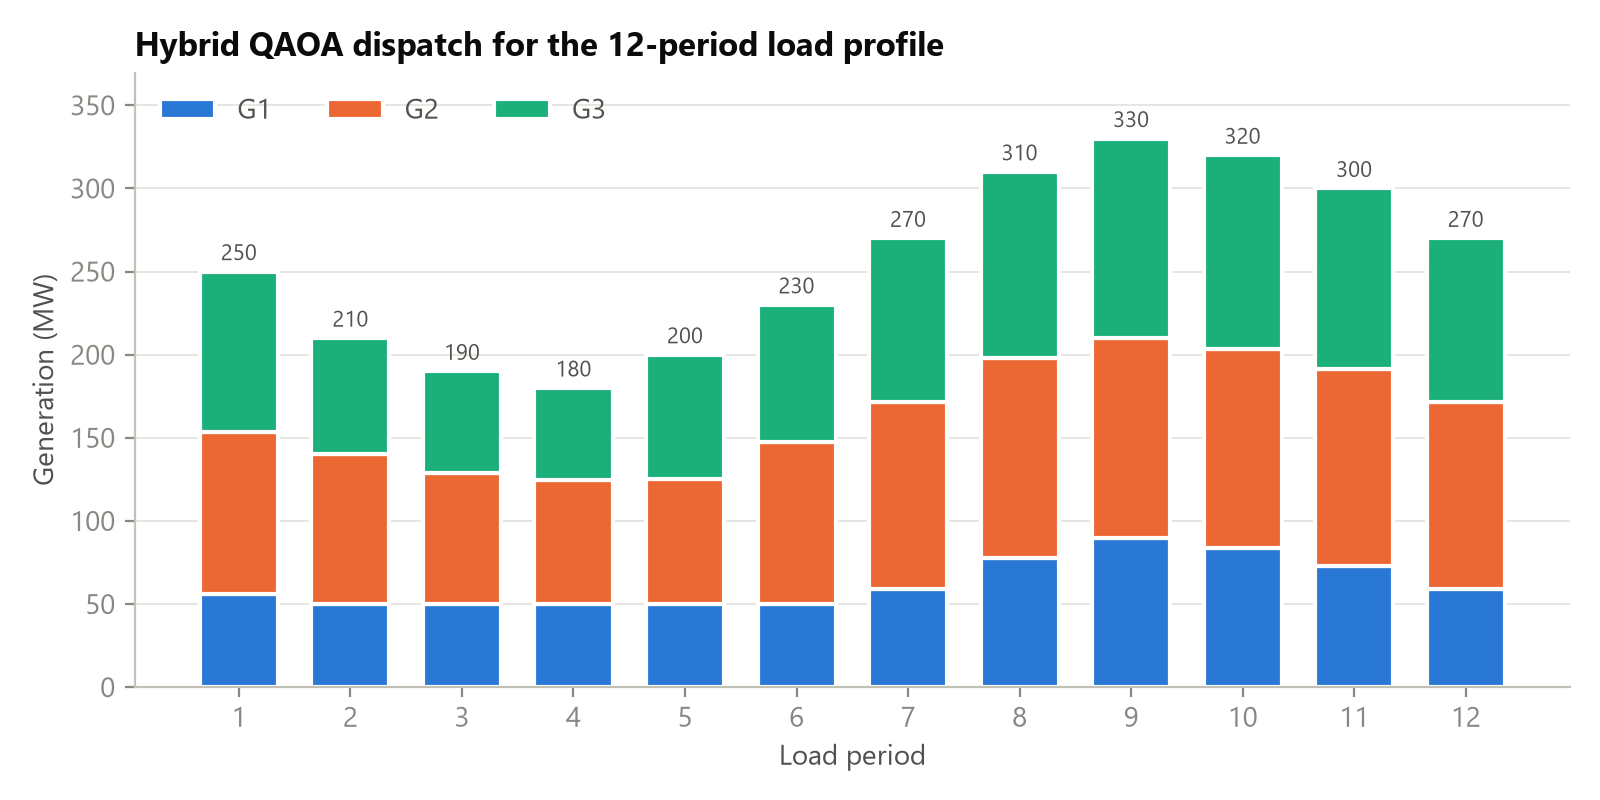
\includegraphics[width=0.92\textwidth]{dispatch_by_period}
\caption{Hybrid QAOA dispatch (12 qubits, $p = 4$, 4096 shots, refinement of the best five bitstrings). Numbers above the bars are the demand in MW.}
\label{fig:dispatch}
\end{figure}

\begin{table}[H]
\centering
\caption{Hybrid QAOA dispatch compared with SLSQP. ``Hits'' is the number of the 4096 shots that returned the exact QUBO optimum.}
\label{tab:hybrid}
\small
\begin{tabular}{ccccrrrc}
\toprule
Period & G1 & G2 & G3 & Hybrid cost & SLSQP cost & Gap (\%) & Hits\\
 & (MW) & (MW) & (MW) & (\$/h) & (\$/h) & & \\
\midrule
1 & 55.89 & 97.50 & 96.61 & 3529.65 & 3528.83 & 0.023 & 1\\
2 & 50.00 & 90.00 & 70.00 & 3046.47 & 3046.41 & 0.002 & 13\\
3 & 50.00 & 78.98 & 61.02 & 2810.05 & 2810.05 & 0.000 & 18\\
4 & 50.00 & 74.44 & 55.56 & 2693.08 & 2693.08 & 0.000 & 34\\
5 & 50.00 & 75.00 & 75.00 & 2929.01 & 2927.83 & 0.040 & 18\\
6 & 50.00 & 97.17 & 82.83 & 3286.01 & 3286.01 & 0.000 & 5\\
7 & 58.80 & 112.50 & 98.70 & 3774.05 & 3774.02 & 0.001 & 4\\
8 & 77.70 & 120.00 & 112.30 & 4269.93 & 4269.91 & 0.000 & 5\\
9 & 90.00 & 120.00 & 120.00 & 4521.12 & 4520.62 & 0.011 & 3\\
10 & 83.52 & 120.00 & 116.48 & 4395.21 & 4395.04 & 0.004 & 12\\
11 & 72.64 & 118.69 & 108.66 & 4145.25 & 4145.25 & 0.000 & 7\\
12 & 58.80 & 112.50 & 98.70 & 3774.05 & 3774.02 & 0.001 & 4\\
\midrule
Total & & & & 43173.88 & 43171.05 & 0.007 & \\
\bottomrule
\end{tabular}
\end{table}

The QUBO optimum was among the measured bitstrings in all 12 periods. After refinement every dispatch meets the demand exactly, and the largest gap is 0.040\,\% (period 5, \$1.18/h). Over the day the hybrid dispatch costs \$2.83 more than the optimum.

The remaining gap is not caused by QAOA. Exhaustive search over all 4096 bitstrings followed by the same refinement gives exactly the same costs (Section~\ref{sec:compare}). It comes from the refinement box: in a few periods the continuous optimum lies more than one grid step from the best grid points. In period 5, for example, the QUBO optimum is (60, 67.5, 72)~MW, while the SLSQP optimum is (50, 83.5, 66.5)~MW; G2 can move only up to 75~MW inside the box, so the refined dispatch stops at (50, 75, 75)~MW.

\section{Cost accuracy and power balance}
Figure~\ref{fig:gap} shows the cost difference of the raw QAOA grid point and of the hybrid dispatch for each period. Some raw grid points appear cheaper than SLSQP; these supply 0.5~MW less than the demand (Figure~\ref{fig:mismatch}) and are not feasible. Refinement removes the mismatch in every period.

\begin{figure}[H]
\centering
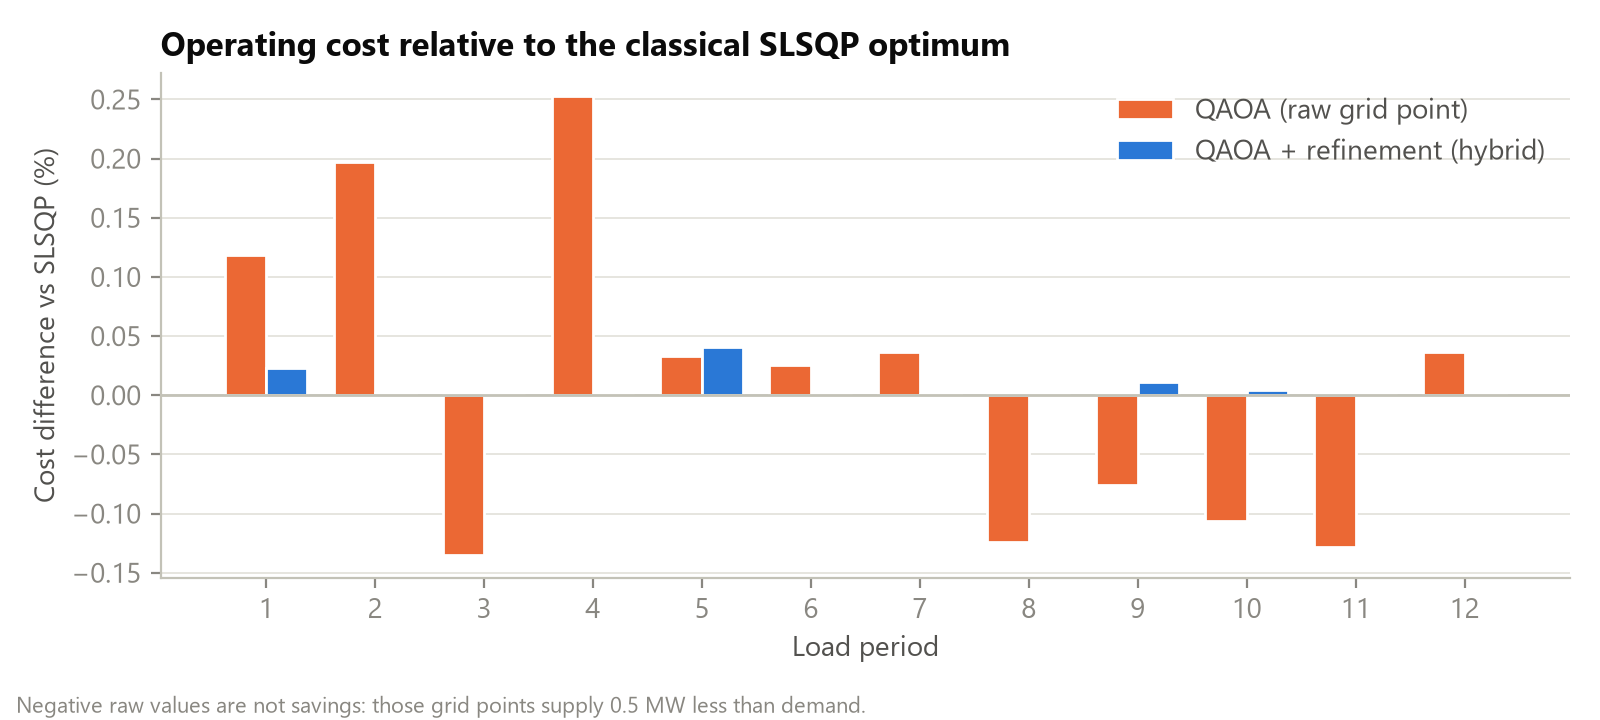
\includegraphics[width=0.92\textwidth]{cost_gap}
\caption{Cost difference relative to SLSQP: raw QAOA grid point and hybrid dispatch.}
\label{fig:gap}
\end{figure}

\begin{figure}[H]
\centering
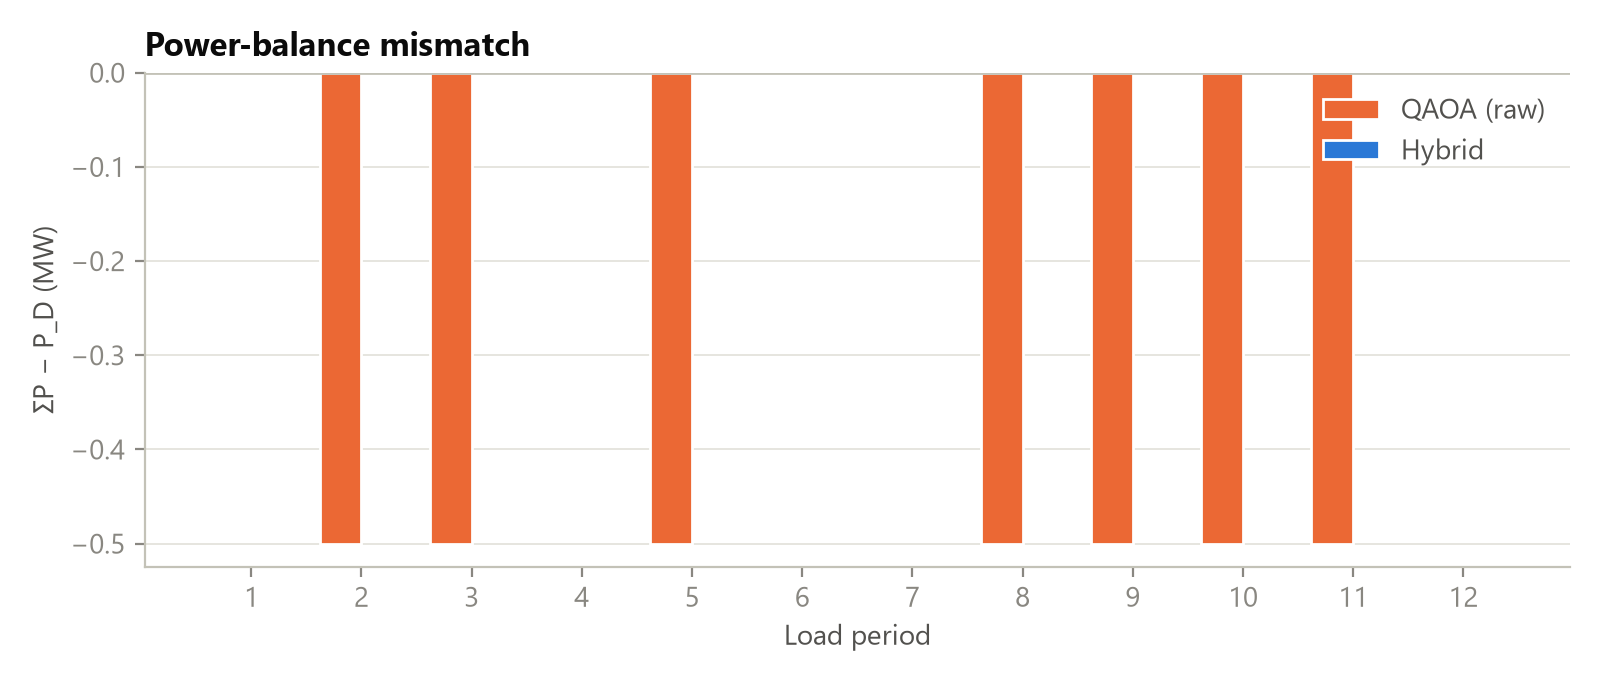
\includegraphics[width=0.92\textwidth]{mismatch}
\caption{Power-balance mismatch $\sum P_i - \PD$ before and after refinement.}
\label{fig:mismatch}
\end{figure}

\section{Effect of circuit depth}
Table~\ref{tab:depth} and Figure~\ref{fig:amp} show how the trained circuit concentrates probability as the depth increases. The amplification of the optimal bitstring rises from 4.6 at $p = 1$ to 10.2 at $p = 4$ on average, and up to 31 in period 4. At $p = 4$, 20.4\,\% of measurements are near-optimal, compared with 3.1\,\% for uniform random sampling (Figure~\ref{fig:pgood}).

\begin{table}[H]
\centering
\caption{QAOA performance against depth (mean over 12 periods; exact statevector).}
\label{tab:depth}
\begin{tabular}{ccccc}
\toprule
$p$ & Amplification & Amplification & Near-optimal & Training\\
 & (mean) & (max) & probability & time (s)\\
\midrule
1 & 4.58 & 15.1 & 10.4\,\% & 3.5\\
2 & 6.76 & 21.3 & 13.9\,\% & 4.0\\
3 & 8.33 & 25.5 & 16.8\,\% & 6.3\\
4 & 10.18 & 31.0 & 20.4\,\% & 8.2\\
\midrule
Random & 1 & 1 & 3.1\,\% & --\\
\bottomrule
\end{tabular}
\end{table}

\begin{figure}[H]
\centering
\begin{minipage}{0.49\textwidth}\centering
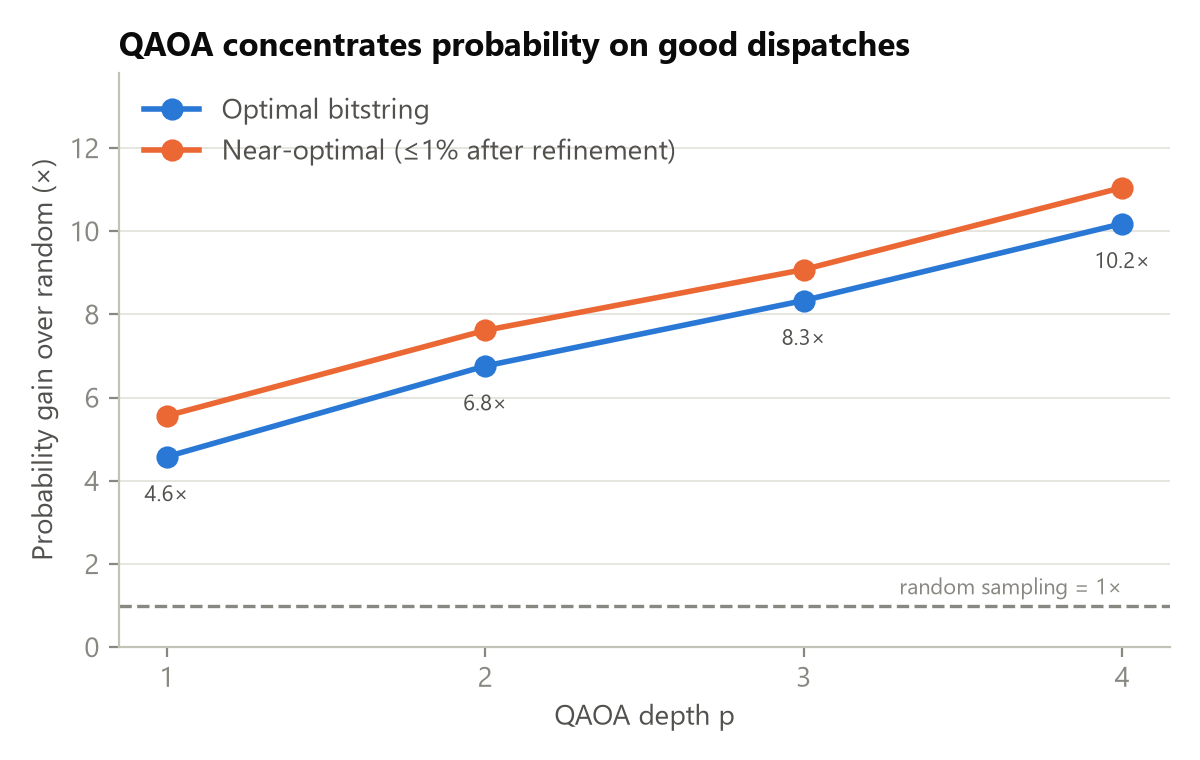
\includegraphics[width=\textwidth]{amplification_vs_depth}
\caption{Probability gain over random sampling against depth.}
\label{fig:amp}
\end{minipage}\hfill
\begin{minipage}{0.49\textwidth}\centering
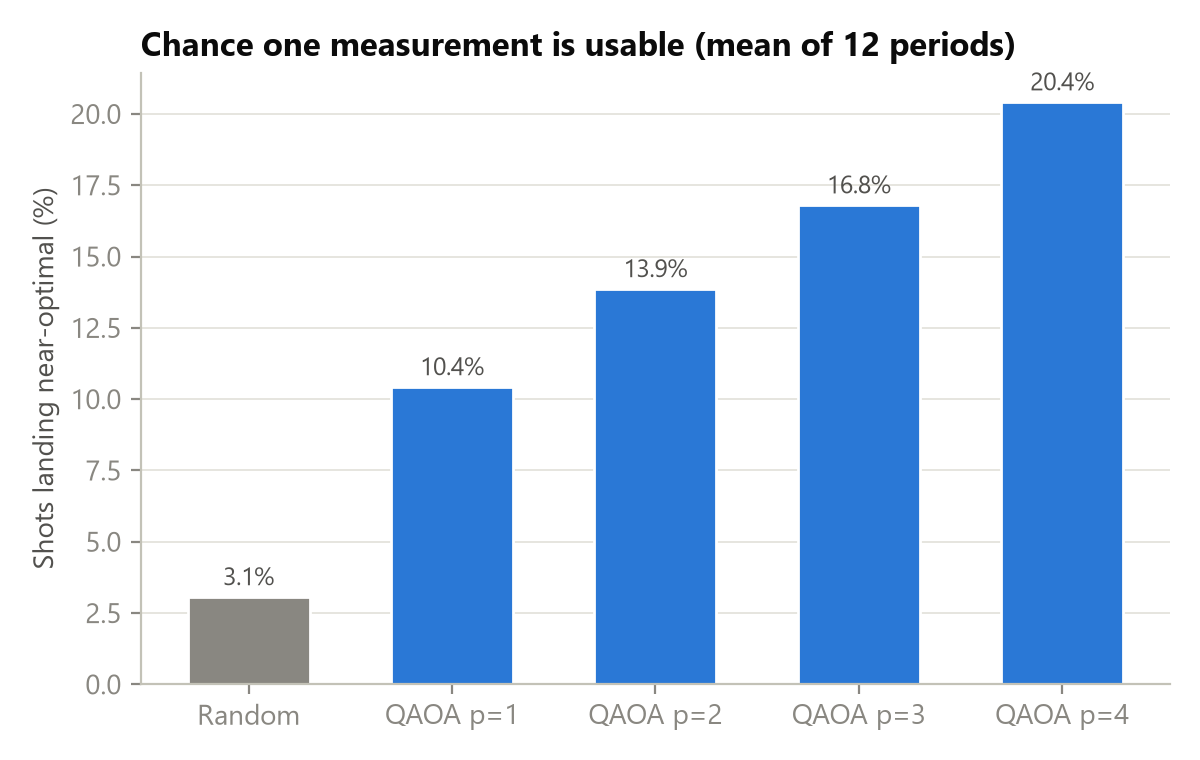
\includegraphics[width=\textwidth]{p_good}
\caption{Chance that one measurement is near-optimal.}
\label{fig:pgood}
\end{minipage}
\end{figure}

The amplification varies strongly between periods: it is highest in periods 2--5 (13.6--31.0 at $p = 4$) and lowest in period 6 (2.4). Figure~\ref{fig:conv} shows the CVaR training curves for period 1 on a logarithmic scale. The $p = 1$ curve (best of eight random starts) begins far from the optimum; the deeper circuits begin from the INTERP extension of the previous optimum, about ten times closer. Depth $p = 4$ reaches the lowest CVaR. In this period $p = 3$ finishes slightly above $p = 2$: COBYLA is a local optimiser, and a single INTERP start does not guarantee monotone improvement. Depths 3 and 4 also use the full 400-iteration budget, so their training time could be reduced with a looser tolerance.

\begin{figure}[H]
\centering
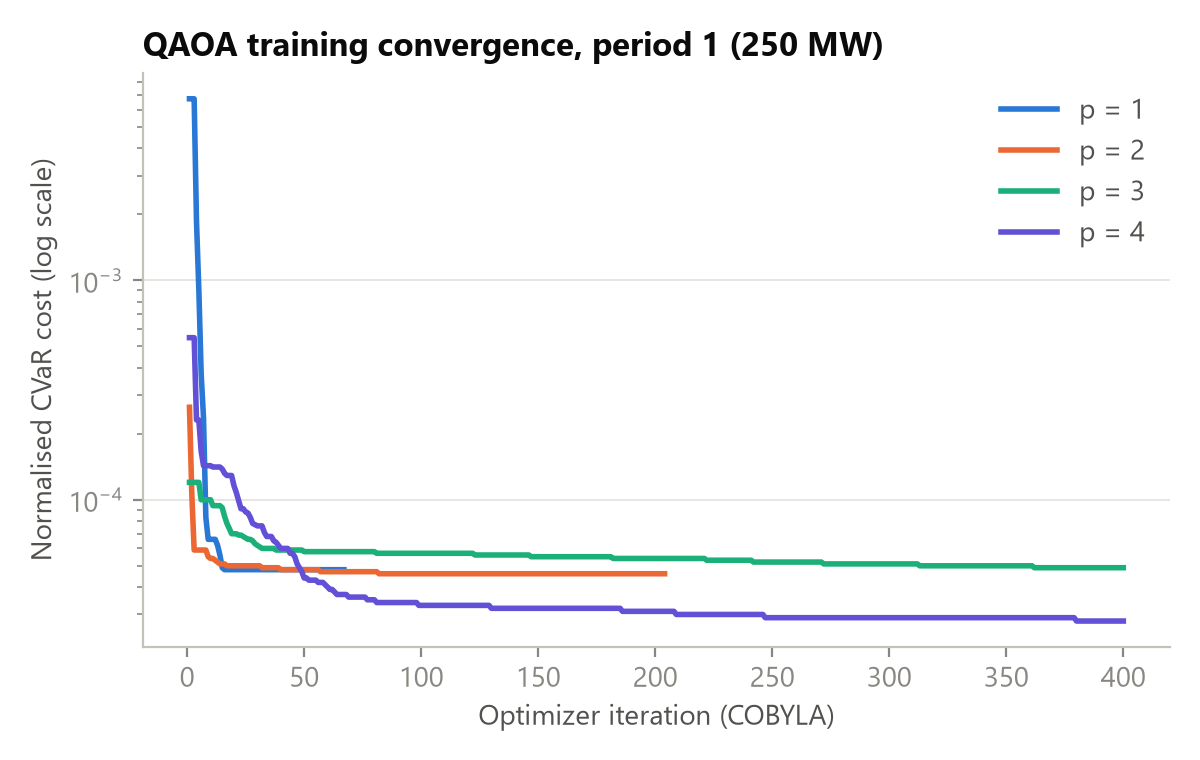
\includegraphics[width=0.7\textwidth]{convergence}
\caption{CVaR training convergence for period 1 (250 MW) at each depth.}
\label{fig:conv}
\end{figure}

\section{Comparison with standard algorithms}
\label{sec:compare}
Table~\ref{tab:compare} compares hybrid QAOA with standard methods over all 12 periods. Every stochastic method was run with 20 random seeds per period (240 runs). Methods that work on the QUBO (exhaustive search, SA and QAOA) all evaluate 4096 bitstrings and refine their five lowest-energy candidates in exactly the same way, so they differ only in how they search the binary space. PSO and GA work on the continuous outputs with a similar budget (3030 evaluations).

\begin{table}[H]
\centering
\caption{Comparison with standard algorithms (12 periods; 20 seeds each for stochastic methods). Success: within 0.1\,\% of SLSQP and $|\text{mismatch}| \le 0.01$~MW.}
\label{tab:compare}
\small
\begin{tabular}{llrrrr}
\toprule
Method & Space & Mean gap & Worst gap & Success & Time/period\\
\midrule
SLSQP (reference) & continuous & 0 & 0 & 100\,\% & 1.3 ms\\
$\lambda$-iteration & continuous & 0 & 0 & 100\,\% & 0.5 ms\\
PSO, dep.\ unit \cite{gaing2003} & continuous & 0.0000\,\% & 0.0003\,\% & 100\,\% & 13 ms\\
GA, dep.\ unit & continuous & 0.0000\,\% & 0.0001\,\% & 100\,\% & 80 ms\\
PSO, penalty & continuous & 0.645\,\% & 2.190\,\% & 13.8\,\% & 10 ms\\
GA, penalty & continuous & 0.763\,\% & 3.011\,\% & 7.5\,\% & 81 ms\\
Exhaustive + refine & 12-bit QUBO & 0.007\,\% & 0.040\,\% & 100\,\% & 10 ms\\
SA + refine & 12-bit QUBO & 0.029\,\% & 0.437\,\% & 92.5\,\% & 71 ms\\
\textbf{QAOA + refine} & 12-bit QUBO & \textbf{0.007\,\%} & \textbf{0.040\,\%} & \textbf{100\,\%} & 0.28 s$^\dagger$\\
\bottomrule
\multicolumn{6}{l}{\footnotesize $^\dagger$ Sampling on a laptop simulator, after about 22~s of training per period.}
\end{tabular}
\end{table}

\begin{figure}[H]
\centering
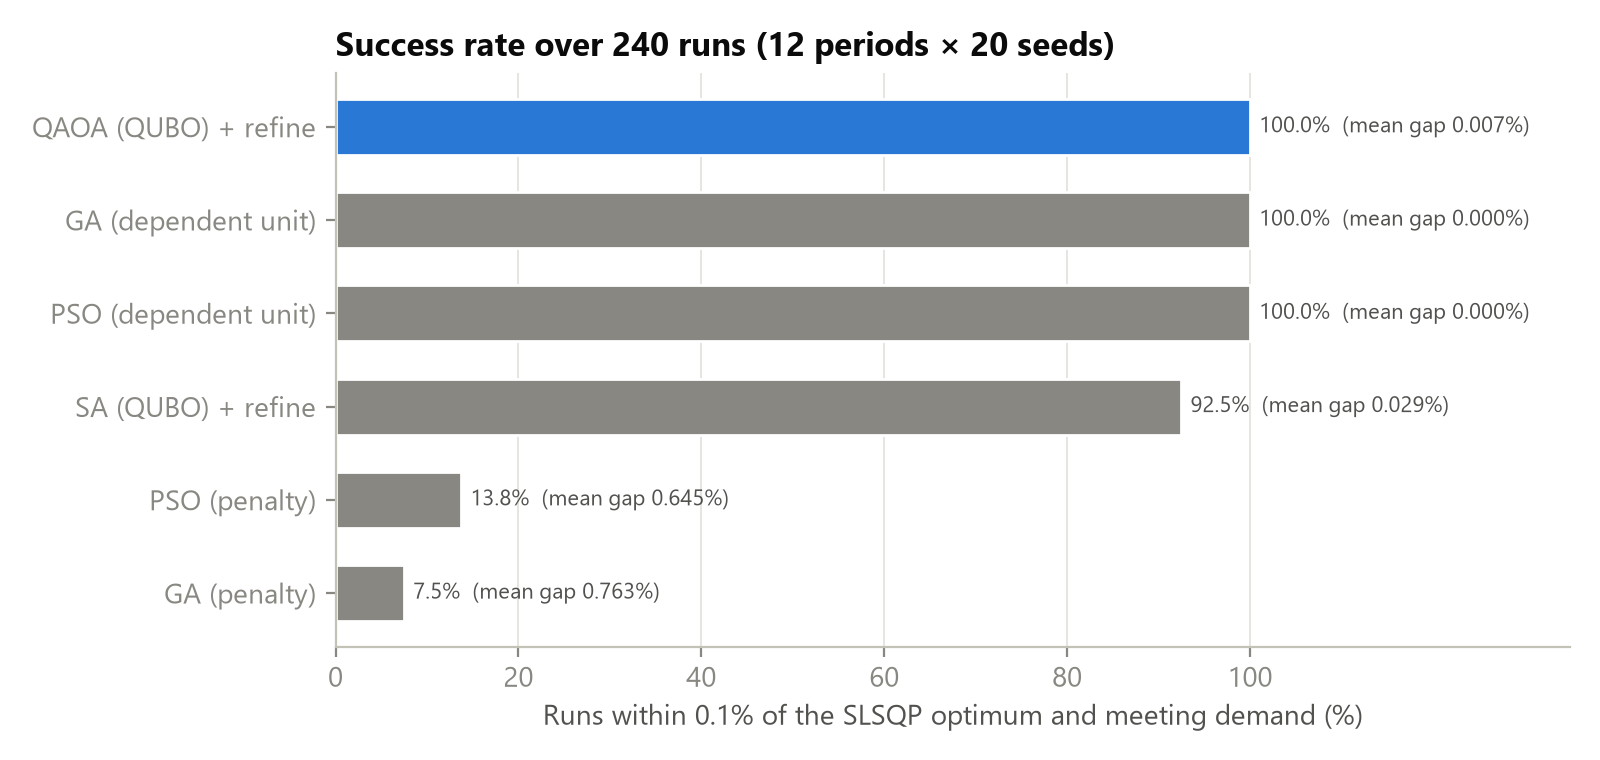
\includegraphics[width=0.9\textwidth]{baselines_success}
\caption{Success rate of the stochastic methods over 240 runs.}
\label{fig:baselines}
\end{figure}

The comparison shows the following.
\begin{itemize}
\item \textbf{Against the same binary problem}, QAOA performed as well as exhaustive search in every one of the 240 runs, with identical costs. Simulated annealing with the same budget and the same refinement succeeded in 92.5\,\% of runs, with a worst gap of 0.44\,\%. On this problem QAOA's sampling was therefore more reliable than SA.
\item \textbf{The 0.007\,\% mean gap of QAOA is a property of the 4-bit grid}, not of QAOA: exhaustive search, which by definition finds the QUBO optimum, gives the same value.
\item \textbf{Continuous heuristics} reach the exact optimum when the balance constraint is handled by the dependent-unit method of Gaing \cite{gaing2003}, because they are not limited to a grid. With a plain penalty they often stop at a nearby but more expensive dispatch (13.8\,\% and 7.5\,\% success). This shows that constraint handling matters as much as the choice of algorithm.
\item \textbf{Speed:} every classical method is faster than simulated QAOA. Simulating a quantum circuit on a classical computer costs time that grows exponentially with the number of qubits, so no runtime advantage can be expected here.
\end{itemize}


\section{Execution on IBM quantum hardware}
Table~\ref{tab:hw} and Figure~\ref{fig:hw} report the hardware experiment on \texttt{ibm\_marrakesh}, a 156-qubit IBM Heron processor (job \texttt{dc299oanj2vs73dgbsd0}, period 1, $p = 1$, 4096 shots).

\begin{table}[H]
\centering
\caption{IBM hardware results, period 1 (250 MW).}
\label{tab:hw}
\begin{tabular}{p{0.42\textwidth}cc}
\toprule
 & 6 qubits (2 bits/unit) & 9 qubits (3 bits/unit)\\
\midrule
Transpiled depth / two-qubit gates & 124 / 46 & 271 / 144\\
P(optimal): random / HW / sim. & 1.56 / 3.69 / 4.11\,\% & 0.20 / 0.24 / 0.53\,\%\\
P(near-opt.): random / HW / sim. & 12.5 / 18.9 / 24.2\,\% & 6.1 / 15.5 / 18.0\,\%\\
QUBO optimum measured on hardware & yes & yes\\
Hybrid cost gap & 0.000\,\% & 0.254\,\%\\
\bottomrule
\end{tabular}
\end{table}

\begin{figure}[H]
\centering
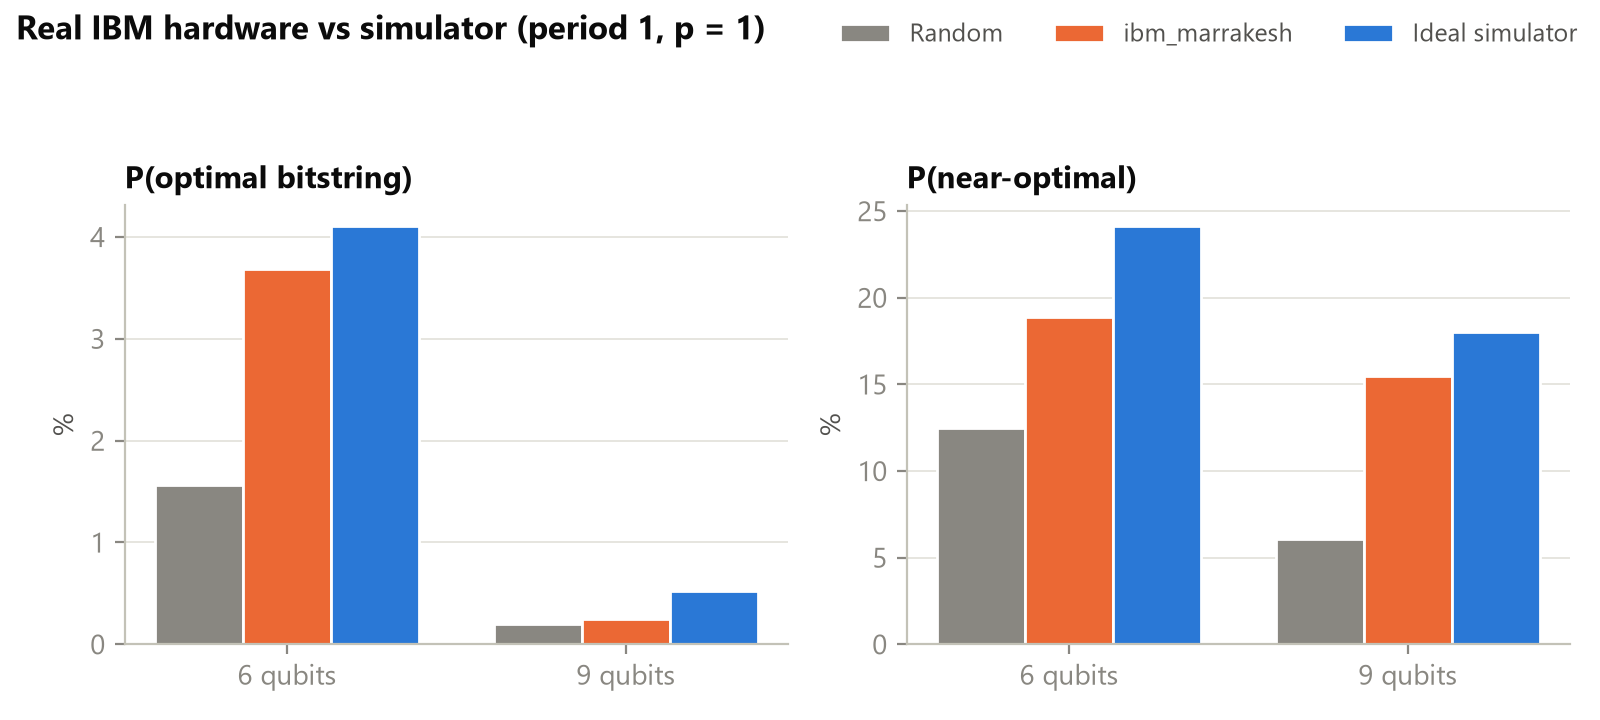
\includegraphics[width=0.9\textwidth]{ibm_hardware}
\caption{Real hardware against the ideal simulator and random sampling.}
\label{fig:hw}
\end{figure}

With 6 qubits, the hardware found the optimal bitstring 2.4 times more often than random sampling and kept about 90\,\% of the ideal simulator's probability; the refined dispatch equals the SLSQP optimum. With 9 qubits, the transpiled circuit needs 144 two-qubit gates, and gate noise reduces the gain on the optimal bitstring to 1.2 times random, although the near-optimal probability (15.5\,\% against 6.1\,\%) still shows a clear signal. The 9-qubit hybrid gap of 0.254\,\% comes from the coarser 3-bit grid (steps of 16--21~MW). These results show that the method runs on present hardware, and that noise, not the formulation, limits the problem size.

\section{Discussion}
\begin{itemize}
\item \textbf{Accuracy.} Hybrid QAOA reaches the SLSQP optimum to within 0.04\,\% in every period; the small remaining gap is set by the binary grid and the refinement box, not by QAOA.
\item \textbf{Quantum effect.} The trained circuit makes the optimal dispatch up to 31 times more likely than random sampling, and the gain grows with depth.
\item \textbf{Speed.} QAOA is not faster. On a laptop the simulator needs about 22~s of training and 0.2~s of sampling per period, while SLSQP needs about 1~ms. For a 3-unit convex problem, classical methods remain the right tool. No quantum speed-up is claimed.
\item \textbf{Where QAOA could help.} The value of the QUBO route lies in problems that are binary by nature, such as unit commitment, where classical solvers face combinatorial growth.
\end{itemize}

\chapter{Transmission Losses and AC Validation}

The lossless model ignores the power dissipated in the lines. This chapter adds losses to the dispatch and checks every dispatch with a full AC load flow, which also reveals the voltages and line loadings that ELD does not model.

\section{Loss formula from the network}
The B-coefficients are derived from the line data rather than taken as given. With bus 1 as the slack, the DC power-transfer distribution factors (PTDF) give the line flows $f = \mathrm{PTDF}\,(C_g P - P_d)$ in per unit, where $C_g$ places each generator at its bus. With voltages close to 1~pu, the losses are $\sum_\ell r_\ell f_\ell^2$. Expanding this square gives Kron's loss formula \cite{wood2014}
\begin{equation}
\PL = P^\top B P + B_0^\top P + B_{00},
\end{equation}
where $B$, $B_0$ and $B_{00}$ depend on the line resistances, the PTDF and the bus loads of the period. The loss-inclusive balance is $\sum_i P_i = \PD + \PL(P)$.

\section{Newton--Raphson AC load flow}
A polar Newton--Raphson load flow with the analytic Jacobian of MATPOWER \cite{matpower2011} was written for the network (lines modelled as $\pi$ sections; bus 1 slack at 1.05~pu; buses 2 and 3 PV at 1.05 and 1.07~pu; loads at power factor 0.98). It was validated against PYPOWER on MATPOWER \texttt{case6ww}: the slack output (107.875~MW), total losses (7.875~MW), generator reactive powers (15.96, 74.36 and 89.63~MVAr) and all bus voltages and angles agree exactly. In this study the load flow converged in 4 iterations in every case.

\section{Hybrid QAOA with losses}
Because the QUBO must be quadratic, the loss term cannot be inserted directly into \eqref{eq:qubo}. An outer iteration is used instead:
\begin{enumerate}
\item Solve the QUBO with QAOA ($p = 3$) for demand $\PD + \PL^{(k)}$, starting with $\PL^{(0)} = 0$.
\item Refine the five best samples with SLSQP subject to the loss-inclusive balance, inside the $\pm1$-step box.
\item Update $\PL^{(k+1)} = \PL(P^{(k)})$ and repeat until the dispatch no longer changes.
\end{enumerate}
The iteration converged in 2 rounds in eleven periods and 3 in period 3.

\section{Results}
\begin{table}[H]
\centering
\caption{Dispatch with losses: costs, losses and AC load-flow checks for the hybrid QAOA dispatch.}
\label{tab:losses}
\small
\begin{tabular}{crrrrrcc}
\toprule
Period & SLSQP & Hybrid & Gap & $\PL$ formula & $\PL$ AC & $V_{\min}$ & T09 loading\\
 & (\$/h) & (\$/h) & (\%) & (MW) & (MW) & (pu) & (\%)\\
\midrule
1 & 3594.48 & 3594.48 & 0.000 & 5.34 & 5.12 & 1.021 & 108\\
2 & 3091.24 & 3091.24 & 0.000 & 3.76 & 3.61 & 1.027 & 89\\
3 & 2846.00 & 2848.25 & 0.079 & 3.12 & 3.05 & 1.030 & 73\\
4 & 2725.09 & 2725.09 & 0.000 & 2.74 & 2.66 & 1.032 & 74\\
5 & 2968.14 & 2968.14 & 0.000 & 3.41 & 3.27 & 1.029 & 84\\
6 & 3341.28 & 3342.01 & 0.022 & 4.59 & 4.41 & 1.024 & 96\\
7 & 3850.57 & 3850.88 & 0.008 & 6.17 & 5.95 & 1.018 & 118\\
8 & 4371.61 & 4371.61 & 0.000 & 8.12 & 7.94 & 1.012 & 134\\
9 & 4636.41 & 4637.13 & 0.016 & 9.17 & 9.03 & 1.009 & 145\\
10 & 4503.80 & 4503.82 & 0.000 & 8.65 & 8.49 & 1.011 & 138\\
11 & 4240.21 & 4240.21 & 0.000 & 7.61 & 7.41 & 1.014 & 130\\
12 & 3850.57 & 3850.88 & 0.008 & 6.17 & 5.95 & 1.018 & 118\\
\midrule
Total & 44019.39 & 44023.73 & 0.010 & 68.83 & 66.90 & & \\
\bottomrule
\end{tabular}
\end{table}

\subsection{Effect of losses on cost}
Losses of 2.7--9.2~MW raise the optimal cost by 1.2--2.6\,\% per period, and by \$848/h (2.0\,\%) over the day. The hybrid QAOA dispatch stays within 0.08\,\% of the loss-inclusive SLSQP optimum in every period, and matches it to within 0.001\,\% in seven of the twelve.

\subsection{Accuracy of the loss formula}
Figure~\ref{fig:losses} compares the formula with the AC load flow. The formula overestimates the losses by 1.5--4.3\,\% because it uses DC flows and ignores reactive power and voltage magnitude. As a result the slack generator in the AC solution produces 0.07--0.22~MW less than scheduled. This error is small compared with the generator ranges, so the formula is adequate for dispatch.

\begin{figure}[H]
\centering
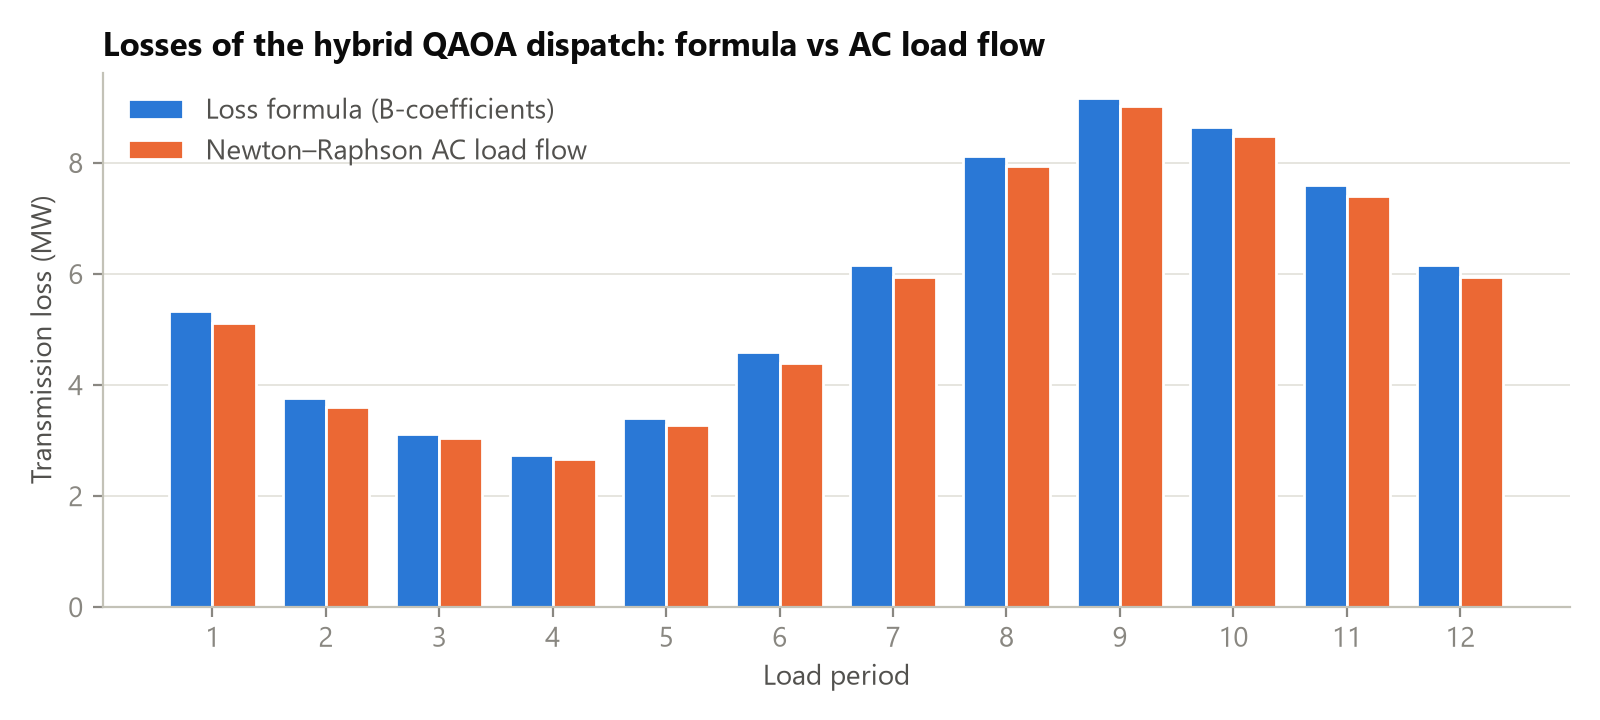
\includegraphics[width=0.9\textwidth]{losses}
\caption{Transmission losses of the hybrid QAOA dispatch: B-coefficient formula against Newton--Raphson.}
\label{fig:losses}
\end{figure}

\subsection{Voltages and reactive power}
All bus voltages stay between 1.009 and 1.070~pu, inside the 0.95--1.07~pu limits, and all generator reactive outputs stay inside their limits in every period.

\subsection{Line loading}
Figure~\ref{fig:lines} shows the loading of line T09 (bus 3 to bus 6), the most heavily loaded line in every period. It exceeds its 60~MVA continuous rating in periods 1 and 7--12, and its 75~MVA short-term rating in periods 8--11, reaching 145\,\% (87~MVA) at the 330~MW peak. The SLSQP optimum produces the same overloads in the same periods (142.7\,\% at the peak), so this is not caused by QAOA: it is a limitation of ELD itself, which ignores the network. G3 at bus 3 is the second-cheapest unit and feeds the load at bus 6 through the low-impedance line T09. Removing the overload requires security-constrained dispatch with line-flow limits, which is proposed as future work.

\begin{figure}[H]
\centering
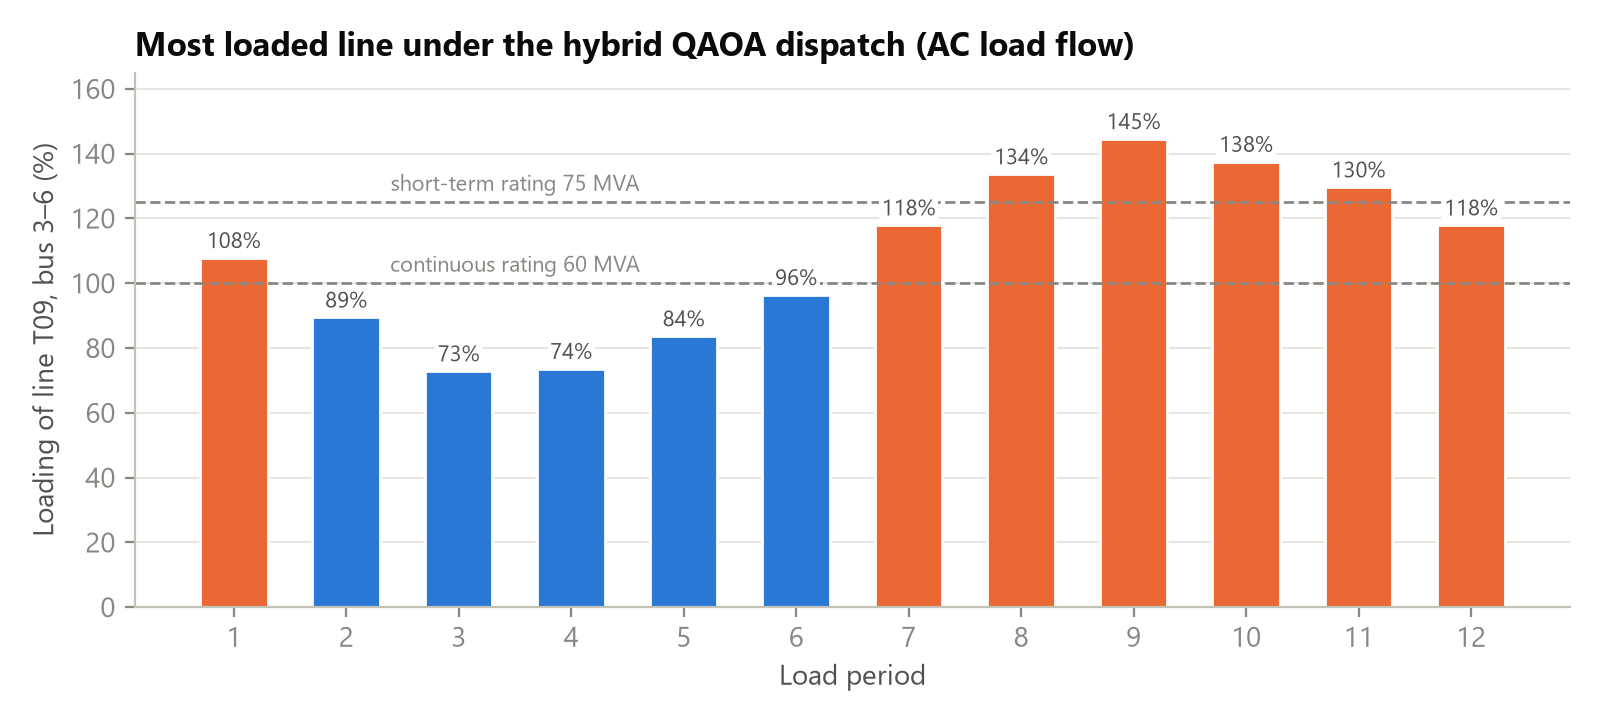
\includegraphics[width=0.9\textwidth]{line_loading}
\caption{Loading of line T09 under the hybrid QAOA dispatch (AC load flow).}
\label{fig:lines}
\end{figure}

\chapter{Conclusion and Future Scope}

\section{Conclusions}
This project formulated the economic load dispatch of the 6-bus, 3-generator system as a 12-qubit QUBO and solved it with QAOA for all 12 periods of a daily load profile. The main conclusions are:
\begin{enumerate}
\item \textbf{Formulation.} Binary encoding with four bits per unit satisfies the generator limits automatically, and a quadratic penalty with $A = 20$, chosen by a sweep, keeps the power mismatch of the QUBO optimum at or below 0.5~MW.
\item \textbf{Accuracy.} QAOA sampled the exact QUBO optimum in all 12 periods. After refinement, the hybrid dispatch meets the demand exactly and is within 0.041\,\% of the SLSQP optimum (\$2.83 over a daily cost of \$43{,}171).
\item \textbf{Quantum effect.} The trained circuit makes the optimal dispatch 10.2 times more likely than random sampling on average at $p = 4$ (up to 31 times), and the gain grows steadily with depth.
\item \textbf{Comparison.} On the same QUBO with the same budget and refinement, QAOA succeeded in 100\,\% of 240 runs, against 92.5\,\% for simulated annealing. Continuous PSO and GA reach the exact optimum only when the balance constraint is handled with the dependent-unit method.
\item \textbf{Hardware.} On IBM \texttt{ibm\_marrakesh}, a 6-qubit instance kept about 90\,\% of the ideal performance and gave the optimal dispatch after refinement; at 9 qubits, noise removed most of the gain.
\item \textbf{Losses and network.} The iterative hybrid method with network-derived B-coefficients stays within 0.08\,\% of the loss-inclusive optimum, and the AC load flow confirms that voltages and reactive powers are within limits. It also shows that line T09 is overloaded at high load for both the quantum and the classical dispatch.
\item \textbf{Speed.} QAOA gives no speed-up: classical methods solve this convex problem in about a millisecond. The project demonstrates correctness and probability amplification, not quantum advantage.
\end{enumerate}

\section{Limitations}
\begin{itemize}
\item The 12-qubit study was simulated; current hardware noise limits real runs to about 6--9 qubits for this circuit.
\item The binary grid needs a classical refinement step to reach the continuous optimum.
\item Single-period ELD only: ramp limits, reserves and unit commitment were not modelled.
\item Line flow limits were checked but not enforced.
\end{itemize}

\section{Future scope}
\begin{itemize}
\item \textbf{Unit commitment}, where the on/off decisions are binary by nature and classical solvers face combinatorial growth: the most promising application of QAOA in power systems.
\item \textbf{Security-constrained dispatch}, adding DC line-flow limits as further penalty terms to remove the T09 overload.
\item \textbf{Larger systems}, such as the IEEE 14- and 30-bus systems, with hardware-efficient encodings.
\item \textbf{Error mitigation} (readout and gate-error mitigation, dynamical decoupling) to extend real hardware runs beyond 9 qubits.
\item \textbf{Multi-period dispatch} with ramp-rate coupling across the 12 periods.
\end{itemize}


\begin{thebibliography}{99}
\addcontentsline{toc}{chapter}{References}

\bibitem{wood2014} A.~J. Wood, B.~F. Wollenberg, and G.~B. Sheblé, \emph{Power Generation, Operation, and Control}, 3rd~ed. Hoboken, NJ, USA: Wiley, 2014.

\bibitem{prada2017} J.~F. Prada, ``Ensuring the reliable operation of the power grid: State-based and distributed approaches to scheduling energy and contingency reserves,'' Ph.D. dissertation, Carnegie Mellon Univ., Pittsburgh, PA, USA, 2017, App.~D.

\bibitem{matpower2011} R.~D. Zimmerman, C.~E. Murillo-Sánchez, and R.~J. Thomas, ``MATPOWER: Steady-state operations, planning, and analysis tools for power systems research and education,'' \emph{IEEE Trans. Power Syst.}, vol.~26, no.~1, pp.~12--19, 2011, doi:10.1109/TPWRS.2010.2051168.

\bibitem{farhi2014} E.~Farhi, J.~Goldstone, and S.~Gutmann, ``A quantum approximate optimization algorithm,'' arXiv:1411.4028, 2014.

\bibitem{lucas2014} A.~Lucas, ``Ising formulations of many NP problems,'' \emph{Front. Phys.}, vol.~2, art.~5, 2014, doi:10.3389/fphy.2014.00005.

\bibitem{barkoutsos2020} P.~Kl. Barkoutsos, G.~Nannicini, A.~Robert, I.~Tavernelli, and S.~Woerner, ``Improving variational quantum optimization using CVaR,'' \emph{Quantum}, vol.~4, p.~256, 2020, doi:10.22331/q-2020-04-20-256.

\bibitem{zhou2020} L.~Zhou, S.-T. Wang, S.~Choi, H.~Pichler, and M.~D. Lukin, ``Quantum approximate optimization algorithm: Performance, mechanism, and implementation on near-term devices,'' \emph{Phys. Rev. X}, vol.~10, 021067, 2020, doi:10.1103/PhysRevX.10.021067.

\bibitem{kraft1988} D.~Kraft, ``A software package for sequential quadratic programming,'' DFVLR, Tech. Rep. DFVLR-FB 88-28, 1988.

\bibitem{gaing2003} Z.-L. Gaing, ``Particle swarm optimization to solving the economic dispatch considering the generator constraints,'' \emph{IEEE Trans. Power Syst.}, vol.~18, no.~3, pp.~1187--1195, 2003, doi:10.1109/TPWRS.2003.814889.

\bibitem{shi1998} Y.~Shi and R.~Eberhart, ``A modified particle swarm optimizer,'' in \emph{Proc. IEEE Int. Conf. Evolutionary Computation}, 1998, pp.~69--73, doi:10.1109/ICEC.1998.699146.

\bibitem{deb1995} K.~Deb and R.~B. Agrawal, ``Simulated binary crossover for continuous search space,'' \emph{Complex Systems}, vol.~9, pp.~115--148, 1995.

\bibitem{kirkpatrick1983} S.~Kirkpatrick, C.~D. Gelatt~Jr., and M.~P. Vecchi, ``Optimization by simulated annealing,'' \emph{Science}, vol.~220, no.~4598, pp.~671--680, 1983, doi:10.1126/science.220.4598.671.

\bibitem{han2024} X.~Han, Z.~Li, and Y.~Xu, ``Quantum assisted stochastic economic dispatch for renewables rich power systems,'' arXiv:2404.13073, 2024.

\bibitem{jing2023} H.~Jing, Y.~Wang, and Y.~Li, ``Data-driven quantum approximate optimization algorithm for power systems,'' \emph{Commun. Eng.}, vol.~2, art.~12, 2023, doi:10.1038/s44172-023-00061-8.

\bibitem{wang2024} M.~Wang, Z.~Cao, and Y.~Li, ``Quantum-behaved particle swarm optimization based on concentration selection probability assignment weights for power system economic dispatch,'' \emph{IEEJ Trans. Electr. Electron. Eng.}, vol.~19, no.~5, pp.~640--652, 2024, doi:10.1002/tee.24015.

\bibitem{qiskit} Qiskit contributors, ``Qiskit: An open-source framework for quantum computing,'' version~2.6.2, 2026. [Online]. Available: https://github.com/Qiskit/qiskit

\end{thebibliography}


\appendix
\chapter{Test-System Data}

\begin{table}[H]
\centering
\caption{Line data (Prada \cite{prada2017}, Table 31), 100~MVA base.}
\label{tab:lines}
\begin{tabular}{lccrrrcc}
\toprule
Line & From & To & $R$ (pu) & $X$ (pu) & $B_c$ (pu) & Rating & Short-term\\
 & & & & & & (MVA) & (MVA)\\
\midrule
T01 & 1 & 2 & 0.10 & 0.20 & 0.04 & 100 & 125\\
T02 & 1 & 4 & 0.05 & 0.20 & 0.04 & 100 & 125\\
T03 & 1 & 5 & 0.08 & 0.30 & 0.06 & 100 & 125\\
T04 & 2 & 3 & 0.05 & 0.25 & 0.06 & 60 & 75\\
T05 & 2 & 4 & 0.05 & 0.10 & 0.02 & 60 & 75\\
T06 & 2 & 5 & 0.10 & 0.30 & 0.04 & 60 & 75\\
T07 & 2 & 6 & 0.07 & 0.20 & 0.05 & 60 & 75\\
T08 & 3 & 5 & 0.12 & 0.26 & 0.05 & 60 & 75\\
T09 & 3 & 6 & 0.02 & 0.10 & 0.02 & 60 & 75\\
T10 & 4 & 5 & 0.20 & 0.40 & 0.08 & 60 & 75\\
T11 & 5 & 6 & 0.10 & 0.30 & 0.06 & 60 & 75\\
\bottomrule
\end{tabular}
\end{table}

\begin{table}[H]
\centering
\caption{Bus and generator operating data.}
\begin{tabular}{lp{0.68\textwidth}}
\toprule
Item & Value (source)\\
\midrule
Base voltage & 230~kV at all buses (Prada Table 30)\\
Voltage limits & 0.95--1.07~pu (Prada Table 30)\\
Bus types & Bus 1 slack, buses 2--3 PV, buses 4--6 PQ (\texttt{case6ww})\\
Voltage set-points & $V_1 = 1.05$, $V_2 = 1.05$, $V_3 = 1.07$~pu (\texttt{case6ww})\\
Reactive limits & G1, G2: $-100$ to $150$~MVAr; G3: $-100$ to $120$~MVAr (Prada Table 33)\\
Base power & 100~MVA (\texttt{case6ww})\\
Load power factor & 0.98 lagging (Prada Sec.~8.1)\\
\bottomrule
\end{tabular}
\end{table}

\chapter{Reproducing the Results}

The code, data, results and this report are in the repository \url{https://github.com/Karthik73965/eld-qaoa}. To reproduce every number:
\begin{lstlisting}
python -m venv .venv
.venv\Scripts\activate          (Windows)   or   source .venv/bin/activate
pip install -r requirements.txt
python tests/test_validation.py      # 4 independent checks
python scripts/run_all.py            # 12-period QAOA study
python scripts/run_penalty_sweep.py
python scripts/run_baselines.py      # PSO, GA, SA, exhaustive, QAOA (20 seeds)
python scripts/run_losses.py         # losses + Newton-Raphson
python scripts/plots.py              # all figures
python scripts/run_ibm.py            # optional: needs IBM_QUANTUM_TOKEN in .env
\end{lstlisting}
The provenance of every input value and the reason for every setting are recorded in \texttt{docs/SOURCES.md}.


\end{document}
